\documentclass[12pt,a4paper]{article}

\renewcommand*\contentsname{Sadržaj}
\renewcommand{\figurename}{Slika}

\usepackage[margin=0.85in]{geometry}
\usepackage{graphicx}
\usepackage{float}
\usepackage{listings}
\usepackage{amsmath}
\usepackage{hyperref}

\renewcommand{\arraystretch}{1.5}
\begin{document}

\begin{titlepage}
	\centering
	{\scshape Univerzitet u Sarajevu \par}
	{\scshape Elektrotehnički Fakultet \par}
	\vspace{1cm}
	{\Large\scshape Prepoznavanje Oblika i Obrada Slike\par}
	\vspace{1.5cm}
	{\huge\bfseries Projektni Zadatak br. 1\par}
	\vspace{2cm}
	\Large Studenti: \par
	{\Large\itshape \textsc{Muftić} Belma, 1423/17260\par}
	{\Large\itshape \textsc{Lemeš} Lamija, 1474/17070\par}
	{\Large\itshape \textsc{Krupalija} Ehlimana, 1431/17461\par}
	\vfill
	Odgovorni asistent:\par
	MoE \textsc{Sumejja Porča}
	\vfill
	{\large Novembar, 2018\par}
\end{titlepage}

\pagenumbering{gobble}

\tableofcontents

\newpage

\pagenumbering{arabic}
\setcounter{page}{1}

\section{\textit{Dataset}}

\subsection{Tema projekta}

Projekat se bavi analizom fotografija različitih vrsta \textbf{krvnih ćelija}. Na slikama se nalaze četiri vrste krvnih ćelija:

\begin{enumerate}

\item \textit{Neutrophil};
\item \textit{Eosinophil};
\item \textit{Monocyte};
\item \textit{Lymphocyte}.

\end{enumerate}

Na slikama je potrebno pronaći ćeliju te odrediti kojoj od sljedećih klasa pripada:

\begin{enumerate}

\item \textit{Neutrophil};
\item \textit{Lymphocyte};
\item Ništa od navedenog (neka druga vrsta krvne ćelije).

\end{enumerate}

Nakon toga potrebno je izdvojiti ćeliju i označiti njenu poziciju na slici.

\subsection{Opis \textit{dataset}-a}

\textit{Dataset} se sastoji od \textbf{12,444} slika. Među tim slikama nalaze se četiri prethodno opisane klase (odnosno vrste krvnih ćelija). Broj uzoraka svake klase prikazan je u sljedećoj tabeli: \\

\begin{center}
\def\arraystretch{1.5}%
\begin{tabular}{| p{3cm} | p{3cm} | p{3cm} | p{3cm} |} \hline

\textbf{Klasa} 						& \textbf{Uzorci za trening}			& \textbf{Uzorci za testiranje}			& \textbf{Ukupan broj uzoraka} 	\\ \hline
\textit{Neutrophil} 					& 2,499								& 624								& 3,123	  						\\ \hline
\textit{Eosinophil} 					& 2,497								& 623								& 3,120	  						\\ \hline
\textit{Monocyte} 					& 2,478								& 620								& 3,098	  						\\ \hline
\textit{Lymphocyte} 					& 2,483								& 620								& 3,103	  						\\ \hline

\end{tabular}
\end{center}

~\\

Za svrhe ovog projekta biti će upotrijebljeno ukupno \textbf{90 slika} (po \textbf{30 slika} za sve tri klase: \textit{Neutrophils}, \textit{Lymhocythes}, ostalo). \\

Cijeli projekat dostupan je na \textit{GitHub}-u, na sljedećem linku: \url{https://github.com/bmuftic1/POOS_Projekat}

\newpage

\section{\textit{DataPrep1}}

Iz foldera \textit{DataSet} učitavaju se slike, jedna po jedna, te se regija od interesa treba označiti tako što se nacrta pravougaonik oko ćelije. Pravougaonik se crta tako što se pritisne na gornji lijevi ugao željene regije, a potom se povuče preko slike sve do donjeg desnog ugla regije od interesa. Kada se to uradi, onda će se pojaviti zeleni pravougaonik, te ako se pritisne \textbf{C}, slika će izdvojiti regiju i nastaviti dalje, a ako se pritisne \textbf{R}, resetuje se slika. Istovremeno se u datoteci \textit{KoordinateROI.txt} pamte koordinate prethodno spomenutih uglova, a struktura datoteke je:

\begin{center}

\texttt{NazivSlike x1,y1,x2,y2}

\end{center}

Slike se spašavaju u folder \textit{ROI}, a kod koji sadrži kreiranje anotacija, kao i slike na kojima je primjenjena maska se nalazi u folderu \textit{Code} pod nazivom \textit{kreiranjeROI.py}. Također, izdvojena je datoteka \textit{spasavanjeSlike.py}, tako da se može koristiti i u narednim zadacima.

\newpage

\section{\textit{DataPrep2}}

\subsection{Uklanjanje šuma}

Za uklanjanje šuma (zamagljivanje slike - \textit{blurring}) izvršen je izbor između sljedećih filtera:

\begin{itemize}

\item \textbf{Filter na bazi prosjeka (\textit{Averaging filter}):} Vrijednost piksela mijenja se sa srednjom vrijednošću svih piksela u oblasti od interesa (na ovaj način zamagljenje slike bude veoma veliko); 
\item \textbf{Filter na bazi statističkog prosjeka (\textit{Mediana filter}):} Vrijednost piksela mijenja se sa medijanom uzorka (efekat zamagljenja je manji);
\item \textbf{Bilateralni filter:} Pri računanju vrijednosti za zamjenu vrši se računanje prosjeka samo za okolinu nekog piksela, što ne uključuje cijelu oblast od interesa (kao rezultat, ivice će biti očuvane, odnosno neće biti zamagljene, dok će se šum smanjiti u ostalim dijelovima slike)

\end{itemize}

Za upotrebu je odabran \textbf{bilateralni filter}, jer iako je sporiji od ostalih filtera, ne zamagljuje ivice, čije je očuvanje važno pri analizi krvnih ćelija. \\

Na sljedećoj slici prikazan je prije i nakon vršenja redukcije šuma korištenjem bilateralnog filtera:

\begin{figure}[H]

\center
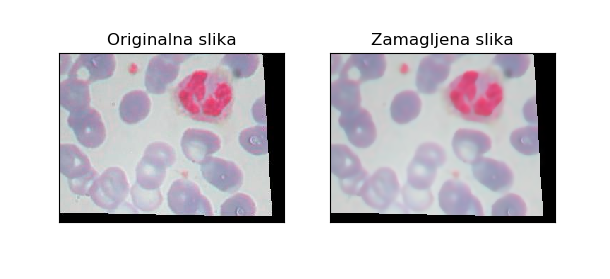
\includegraphics[scale=0.9]{s1SmanjenjeSuma.png}
\caption{Smanjenje šuma na slici korištenjem bilateralnog filtera}

\end{figure}

\newpage

\subsection{Maskiranje neoštrina}

Za maskiranje neoštrina izabrana je kernel matrica sa vrijednostima:
\[
\begin{bmatrix}
    0 & -2 & 0 \\
    -2 & 9 & -2 \\
    0 & -2 & 0
\end{bmatrix}
\]

Na slici ispod prikazan je rezultat izoštravanja u odnosu na originalnu sliku:


\begin{figure}[H]

\center
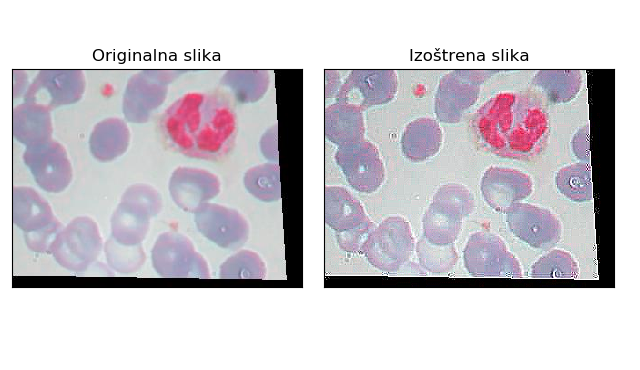
\includegraphics[scale=0.9]{s2MaskiranjeNeostrina.png}
\caption{Izoštravanje slike korištenjem filtera za maskiranje neoštrina}
	
\end{figure}

\newpage

\section{\textit{DataPrep3}}

\subsection{Poboljšavanje kvaliteta slika}

\subsubsection{Poboljšavanje kontrasta}

Za poboljšavanje kontrasta slike korištena su tri različita postupka, koji će biti opisani u nastavku.

\begin{enumerate}

\item \textbf{Aritmetičke operacije}: \\

Kako bi se poboljšao kontrast slike, prvenstveno je neophodno pretvoriti RGB u HLS sliku. Zatim se vrši manipulacija nad pikselima koji označavaju \textit{Luminence} u okviru tako transformisane slike. Koriste se aritmetičke operacije nad pojedinačnim pikselima slike, na sljedeći način:

\begin{itemize}

\item Ukoliko je vrijednost piksela manja od srednje vrijednosti svih \textit{Luminence} piksela, vrši se \textbf{smanjenje vrijednosti piksela} za iznos faktora koji se može prilagođavati (svijetli pikseli postaju svjetliji za iznos faktora);
\item Ukoliko je vrijednost piksela veća od srednje vrijednosti svih \textit{Luminence} piksela, vrši se \textbf{povećanje vrijednosti piksela} za iznos faktora koji se može prilagođavati (tamni pikseli postaju tamniji za iznos faktora).

\end{itemize}

Na sljedećoj slici prikazan je izgled slike prije i nakon vršenja poboljšanja za vrijednost faktora \texttt{factor = 30}:

\begin{figure}[H]

\center
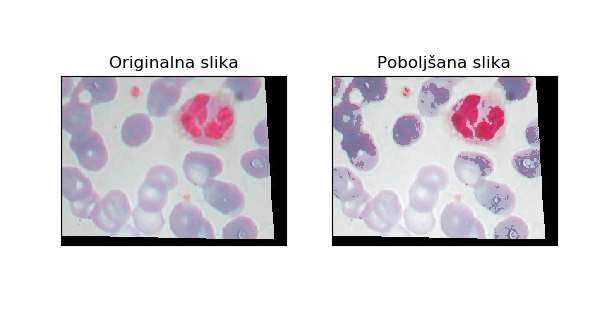
\includegraphics[scale=0.9]{s3Kontrast1.png}
\caption{Poboljšavanje kontrasta slike korištenjem aritmetičkih operacija}

\end{figure}

\newpage

\item \textbf{Linearno razvlačenje kontrasta}: \\

Drugi metod poboljšanja kontrasta slike postiže se manipulacijom nad pojedinačnim kanalima slike. Svaka vrijednost piksela se određuje u zavisnosti od vrijednosti susjednih piksela. Intenzitet se izračunava pomoću formule za normalizaciju:

\[
	I_o = (I_i - Min_i) * (((Max_o - Min_o) / (Max_i - Min_i)) + Min_o)
\]

Gdje su vrijednosti:

\begin{itemize}

\item \texttt{I$_o$} - Izlazna vrijednost piksela
\item \texttt{I$_i$} - Ulazna vrijednost piksela
\item \texttt{Min$_i$} - Minimalna vrijednost piksela u ulaznoj slici
\item \texttt{Max$_i$} - Maksimalna vrijednost piksela u ulaznoj slici
\item \texttt{Min$_o$} - Minimalna vrijednost piksela u izlaznoj slici
\item \texttt{Max$_o$} - Maksimalna vrijednost piksela u izlaznoj slici

\end{itemize}

Na sljedećoj slici prikazan je izgled slike prije i nakon linearnog razvlačenja kontrasta:

\begin{figure}[H]

\center
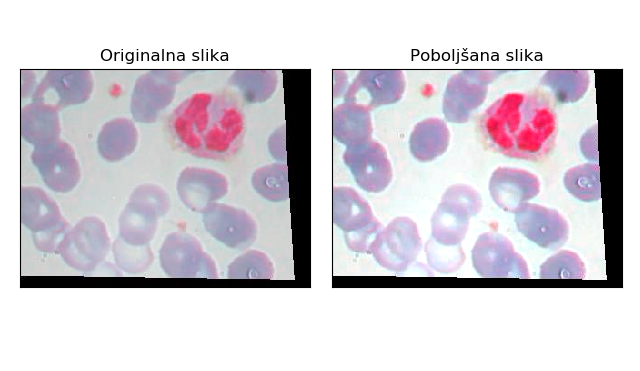
\includegraphics[scale=0.9]{s4Kontrast2.png}
\caption{Poboljšavanje kontrasta slike korištenjem linearnog razvlačenja}
	
\end{figure}

\newpage

\item \textbf{\textit{Gamma} korekcija}: \\

Za ovaj zadatak korištena je \textit{gamma} korekcija koja transformiše datu sliku prema formuli:

\[NovaSlika = Slika^{\frac{1}{gamma}}\]

gdje je \texttt{gamma} vrijednost koju mi zadajemo. \\

Novu sliku je potrebno korigovati tako da su vrijednosti piksela u opsegu 0 do 255, uključivo. Za vrijednost \texttt{gamma} je odabrano 0.7, kako se treba istaći ljubičasti dio regije od interesa. Samo računanje novih vrijednosti piksela je urađeno preko LUT (\textit{lookup table}), gdje su se pikseli originalne slike mapirali u piksele \texttt{gamma} korigovane slike prema navedenoj formuli. Rezultat poboljšanja kontrasta je prikazan na sljedećoj slici:

\begin{figure}[H]

\center
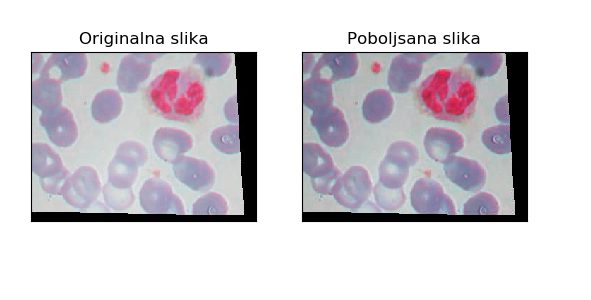
\includegraphics[scale=0.9]{s5Kontrast3.png}
\caption{Poboljšavanje kontrasta slike korištenjem \textit{gamma} korekcije}
	
\end{figure}

\end{enumerate}

\newpage

\subsubsection{Povećanje osvjetljenja}

Za povećanje osvjetljenja slike korištena su tri različita postupka, koji će biti opisani u nastavku.

\begin{enumerate}

\item \textbf{Aritmetičke operacije}: \\

Kako bi se povećalo osvjetljenje slike, prvenstveno je neophodno pretvoriti RGB u HLS sliku. Zatim se vrši manipulacija nad pikselima koji označavaju \textit{Luminence} u okviru tako transformisane slike. Koristi se aritmetička operacija \textbf{sabiranja} pojedinačnih piksela slike sa iznosom faktora (koji se može prilagođavati).


Na sljedećoj slici prikazan je izgled slike prije i nakon vršenja poboljšanja za vrijednost faktora \texttt{factor = 30}:

\begin{figure}[H]

\center
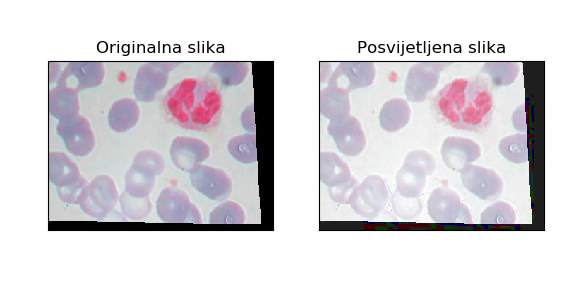
\includegraphics[scale=0.9]{s6Osvjetljenje1.png}
\caption{Povećanje osvjetljenja slike korištenjem aritmetičke operacije sabiranja}

\end{figure}

\newpage

\item \textbf{Linearne transformacije}: \\

Drugi metod za povećanje osvjetljenja slike podrazumijeva primjenu linearnih transformacija. Konkretno promjena vrijednosti parametra beta u OpenCV funkciji \textit{convertScaleAbs}.

Na sljedećoj slici je izgled slike prije i nakon povećanja osvjetljenja postavljanjem vrijednosti parametra \texttt{beta} na 20 (moguće su vrijednosti od 0 do 100):

\begin{figure}[H]

\center
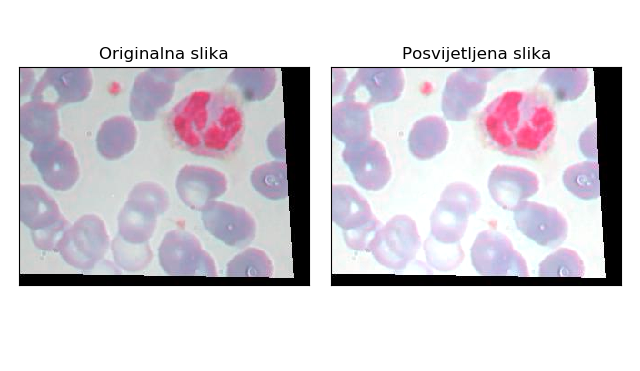
\includegraphics[scale=0.9]{s7Osvjetljenje2.png}
\caption{Povećanje osvjetljenja slike korištenjem linearne transformacije}
	
\end{figure}

\newpage

\item \textbf{Manipulacija HSV slike}: \\

Korištena je manipulacija intenziteta treće komponente HSL-a, tj. \textit{lightness}. Faktor kojim se poboljšava osvjetljenje je 40, te u slučaju da zbir trenutne vrijednosti treće komponente piksela i faktora ima vrijednost veću od 255, vrijednost se postavlja na 255, u suprotnom, nova vrijednost postaje pomenuti zbir. Nakon korekcije treće komponente, sve tri komponente se spajaju u HSV sliku, koja se zatim pretvori u BGR vrijednost, i spasi u folder \textit{Brightness}. Sljedeća slika prikazuje promjenu osvjetljenja odabrane slike pomoću manipulacije HSV:

\begin{figure}[H]

\center
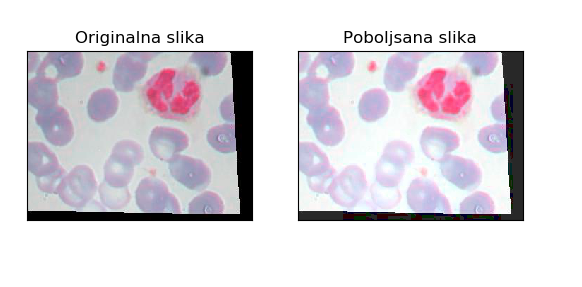
\includegraphics[scale=0.9]{s8Osvjetljenje3.png}
\caption{Povećanje osvjetljenja slike korištenjem manipulacije HSV slike}
	
\end{figure}

\end{enumerate}

\newpage

\subsubsection{Ujednačavanje histograma}

Za ujednačavanje histograma slike korištena su tri različita postupka, koji će biti opisani u nastavku.

\begin{enumerate}

\item \textbf{Raspodjela vjerovatnoća}: \\

Kako bi se ujednačio histogram slike, prvenstveno je neophodno pretvoriti RGB u HLS sliku. Zatim se vrši analiza piksela koji označavaju \textit{Luminence} u okviru tako transformisane slike. Za svaki piksel pronalazi se njegova okolina (čija veličina ovisi o iznosu prilagodljivog faktora), te se zatim pronalazi vrijednost \textbf{piksela s najmanjom frekvencijom pojavljivanja} iz te okoline. Zatim se trenutni piksel izjednačava s tom vrijednošću i vrijednost frekvencije piksela povećava. Na ovaj način postiže se ujednačavanje histograma, odnosno preraspodjela vjerovatnoće pojavljivanja piksela u okolinu. \\

Na sljedećoj slici prikazan je izgled slike i njenog pripadajućeg histograma prije i nakon vršenja ujednačavanja histograma za vrijednost faktora \texttt{factor = 30}:

\begin{figure}[H]

\center
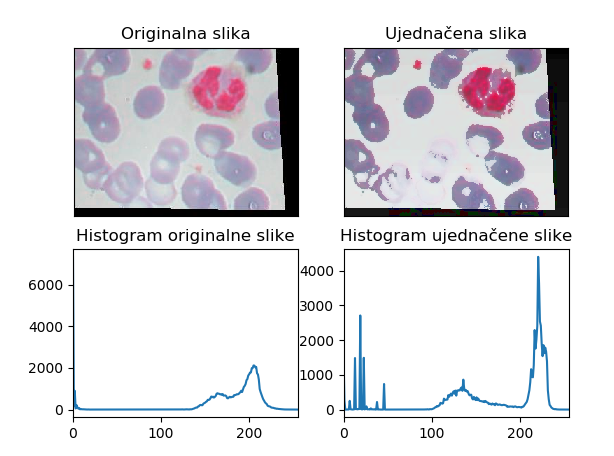
\includegraphics[scale=0.9]{s9Histogram1.png}
\caption{Ujednačavanje histograma slike korištenjem raspodjele vjerovatnoća}

\end{figure}

\newpage

\item \textbf{CLAHE}: \\

Drugi metod ujednačavanja histograma slike jeste CLAHE (eng. \textit{Contrast Limited Adaptive Histogram Equalization}). Da bi se omogućilo korištenje ovog tipa ujednačavanja, sliku je bilo potrebno prethodno pretvoriti u \textit{grayscale}.

Na sljedećoj slici prikazan je izgled slike i njenog histograma prije i nakon izvršenja ujednačavanja histograma za vrijednost faktora \texttt{factor = 10}:

\begin{figure}[H]

\center
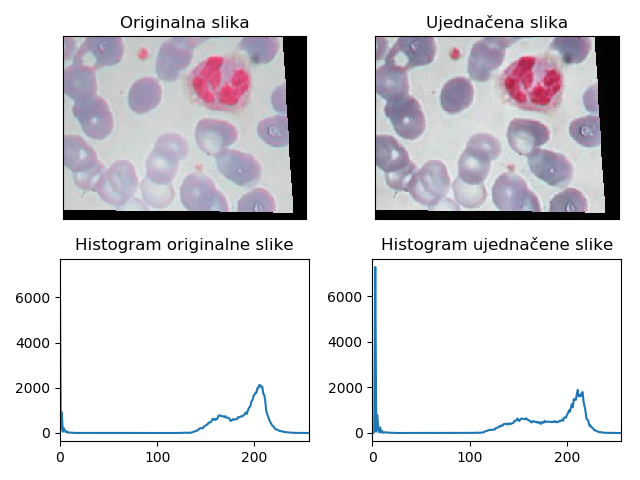
\includegraphics[scale=0.9]{s10Histogram2.png}
\caption{Ujednačavanje histograma slike korištenjem CLAHE}
	
\end{figure}

\newpage

\item \textbf{\texttt{equalizeHist}}: \\

Za ujednačavanje histograma korištena je funkcija \texttt{equalizeHist} iz biblioteke cv2, i to nad svim \textit{channels} od date RGB slike, nakon čega je ista spašena u folder \textit{Histogram}. Na sljedećoj slici je prikazan rezultat primjene ove funkcije:

\begin{figure}[H]

\center
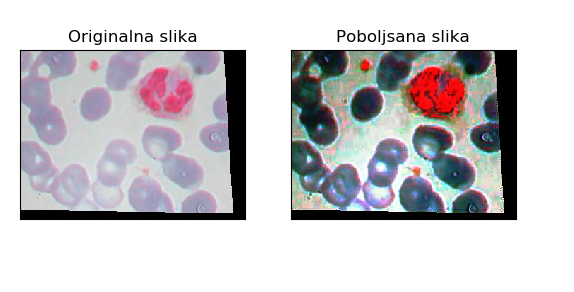
\includegraphics[scale=0.9]{s11Histogram3.png}
\caption{Ujednačavanje histograma slike korištenjem \texttt{equalizeHist}}
	
\end{figure}

\end{enumerate}

\newpage

\section{\textit{DataPrep4}}

Kreiran je file \textit{podjela.py} koji definiše kako će se \textit{dataset} podijeliti, gdje je odlučeno da podjela bude sljedeća:

\begin{itemize}

\item \textbf{Validacija (10\%)}: Po 3 slike za svaku klasu, dakle ukupno 9 slika;
\item \textbf{Test (25\%)}: Po 7 slika za svaku klasu, dakle ukupno 21 slika;
\item \textbf{Trening (65\%)}: Po 19 slika za svaku klasu, dakle ukupno 60 slika.

\end{itemize}

Kako su slike poredane tako da se one sa brojevima između 1 i 30 uključivo nalaze u prvoj klasi, one sa brojevima između 31 i 60 u drugoj klasi, a slike sa brojevima u nazivu između 61 i 90 pripadaju klasi tri, tako je moguće izvršiti ravnopravnu podjelu tako da svaka klasa bude zastupljena u svakom skupu. Prvo se kreiraju folderi \textit{Validacija}, \textit{Test} i \textit{Train} (u slučaju da već ne postoje), te se nasumice generišu brojevi između prethodno spomenutih intervala. Slike sa datim brojem se potom kopiraju u odgovarajući folder. Dovoljno je samo pokrenuti datoteku, bez poziva funkcija, kako se kod nalazi u \texttt{main} funkciji. \\

Također, važno je naznačiti da se svaka \textit{.py} datoteka može uključiti kao \textit{.dll} i nije potrebno pozivati određene funkcije unutar njih, već samo pozvati sami modul, te će on izvršiti ono što se nalazi u \texttt{main} funkciji (primjer upotrebe se nalazi u \textit{projekat.py}).

\end{document}